\documentclass[a4paper]{oblivoir}
\usepackage{amsmath,amssymb,kotex,kswrapfig,mdframed,paralist}
\usepackage{fapapersize}
\usefapapersize{210mm,297mm,10mm,*,10mm,*}

\usepackage{tabto,pifont}
\TabPositions{0.2\textwidth,0.4\textwidth,0.6\textwidth,0.8\textwidth}
\newcommand\tabb[5]{\par\noindent
\ding{172}\:{\ensuremath{#1}}
\tab\ding{173}\:\:{\ensuremath{#2}}
\tab\ding{174}\:\:{\ensuremath{#3}}
\tab\ding{175}\:\:{\ensuremath{#4}}
\tab\ding{176}\:\:{\ensuremath{#5}}}

\usepackage{graphicx}

\pagestyle{empty}

%%% Counters
\newcounter{num}

%%% Commands
\newcommand\prob[1]
{\vs\bigskip\par\noindent\stepcounter{num} \textbf{문제 \thenum) #1}\par\noindent}

\newcommand\pb[1]{\ensuremath{\fbox{\phantom{#1}}}}

\newcommand\ba{\ensuremath{\:|\:}}

\newcommand\vs[1]{\vspace{60pt}}

\newcommand\an[1]{\bigskip\par\noindent\textbf{문제 #1)}\par\noindent}

%%% Meta Commands
\let\oldsection\section
\renewcommand\section{\clearpage\oldsection}

\let\emph\textsf

\begin{document}
\begin{center}
\LARGE수지, 추가과제 06
\end{center}
\begin{flushright}
날짜 : 2017년 \(\pb3\)월 \(\pb{10}\)일 \(\pb{월}\)요일
,\qquad
제한시간 : \pb{17년}분
,\qquad
점수 : \pb{20} / \pb{20}
\end{flushright}

%
\prob{}
다음 극한값을 구하여라.
\par\bigskip\noindent
(1) \(\displaystyle\lim_{x\to0}\frac{6x+5x^2}{2x-3x^2}\)
\tabto{0.33\textwidth}
(2) \(\displaystyle\lim_{x\to1}\frac{2x^2-3x+1}{x^2-1}\)
\tabto{0.66\textwidth}
(3) \(\displaystyle\lim_{x\to0}\frac{x}{\sqrt{x+1}-1}\)
\par\bigskip\noindent
(4) \(\displaystyle\lim_{x\to-\infty}(x^4-3x^3+4)\)
\tabto{0.33\textwidth}
(5) \(\displaystyle\lim_{x\to\infty}\left(\sqrt{4x^2+3x-1}-2x\right)\)
\tabto{0.66\textwidth}
(6) \(\displaystyle\lim_{x\to0}\frac1x\left\{1-\frac1{(x+1)^2}\right\}\)
\par\bigskip\noindent
(7) \(\displaystyle\lim_{x\to\infty}\left(\sqrt{x+1}-\sqrt x\right)\)
\tabto{0.33\textwidth}
(8) \(\displaystyle\lim_{x\to0}\frac1x\left(\frac1{x+1}-1\right)\)
\tabto{0.66\textwidth}
(9) \(\displaystyle\lim_{x\to0}\frac1x\left\{\frac1{\sqrt3-x}-\frac1{\sqrt3}\right\}\)
\par\bigskip

%
\prob{}
다음 중 그 값이 가장 큰 것은? 
(단, \([x]\)는 \(x\)보다 크지 않은 최대의 정수이다.)\par\bigskip
\tabb
{\displaystyle\lim_{x\to0-}\frac{x}{[x]}}
{\displaystyle\lim_{x\to0+}\frac{[x]}{x}}
{\displaystyle\lim_{x\to0-}\frac{[x-1]}{x-1}}
{\displaystyle\lim_{x\to0+}\frac{x+1}{[x+1]}}
{\displaystyle\lim_{x\to3+}\frac{[x-3]}{x-3}}

%
\prob{}
함수 \(f(x)\), \(g(x)\)가
\[\lim_{x\to\infty}f(x)=\infty,\qquad\lim_{x\to\infty}\left\{3f(x)-2g(x)\right\}=1\]
을 만족시킬 때, \(\displaystyle\lim_{x\to\infty}\frac{f(x)+4g(x)}{-2f(x)+6g(x)}\)의 값을 구하여라.

%
\prob{}
함수 \(f(x)\)에 대하여 \(\displaystyle\lim_{x\to0}\frac{f(x)}{x}=3\)일 때, \(\displaystyle\lim_{x\to2}\frac{f(x-2)}{x-2}\)의 값을 구하여라.

%
\prob{}
다음 함수의 \(x=1\)에서의 연속성을 조사하여라.
(단 \([x]\)는 \(x\)보다 크지 않은 최대의 정수이다.)
\par\bigskip\noindent
(1) \(f(x)=\begin{cases}\displaystyle\frac{x^2+2x-3}{x-1}&(x\neq1)\\4&(x=1)\end{cases}\)
\tabto{0.5\textwidth}
(2) \(f(x)=x-[x]\)
\par\bigskip

%
\prob{}
\begin{minipage}{0.5\textwidth}
함수 \(y=f(x)(-1<x<4)\)의 그래프가 오른쪽 그림과 같다.
함수 \(f(x)\)의 극한값이 존재하지 않는 점의 개수를 \(a\)개, 불연속인 점의 개수를 \(b\)개라 할 때, \(a+b\)의 값을 구하여라.
\end{minipage}
\begin{minipage}{0.3\textwidth}
\par\bigskip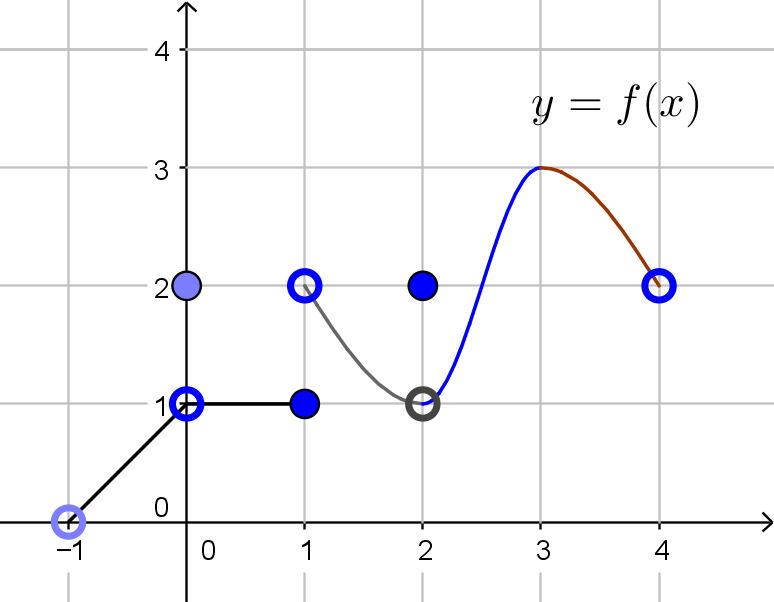
\includegraphics[width=0.6\textwidth]{fx}
\end{minipage}\bigskip\bigskip\par

%
\prob{}
함수 \(f(x)=\begin{cases}\displaystyle\frac{x^2+ax+b}{x+2}&(x\neq-2)\\5&(x=-2)\end{cases}\)가 \(x=-2\)에서 연속이 되도록 하는 상수 \(a\), \(b\)의 값을 각각 구하여라.

%
\prob{}
모든 실수 \(x\)에 대하여 연속인 함수 \(f(x)\)가
\[(x-2)f(x)=x^2+ax-12\]
를 만족시킬 때, 상수 \(a\)의 값과 \(f(2)\)의 값을 구하여라.

%
\prob{}
두 함수 \(f(x)=x^2-3\), \(g(x)=x^2-4x-5\)에 대하여 다음 함수가 연속인 \(x\)의 값의 범위를 구간의 기호를 써서 나타내어라.
\par\bigskip\noindent
(1) \(f(x)-3g(x)\)
\tabto{0.25\textwidth}
(2) \(f(x)g(x)\)
\tabto{0.5\textwidth}
(3) \(\displaystyle\frac{f(x)}{g(x)}\)
\tabto{0.75\textwidth}
(4) \(\displaystyle\frac1{f(x)-g(x)}\)
\par\bigskip

%
\prob{}
주어진 구간에서 다음 함수 \(f(x)\)의 최댓값과 최솟값을 각각 구하여라.
\par\bigskip\noindent
(1) \(f(x)=-x^2+2x+3,\qquad[-2,2]\)
\par\bigskip\noindent
(2) \(f(x)=\frac2{x-2},\qquad[3,5]\)
\par\bigskip

%
\prob{}
방정식 \(x^3-2x^2-1=0\)이 열린구간 \((2,3)\)에서 적어도 하나의 실근을 가짐을 보여라.

\end{document}